\documentclass[12pt]{article}
\usepackage{tikz}
\usepackage{xspace}
\pagestyle{empty}
\textwidth      165mm
\textheight     252mm
\topmargin      -18mm
\oddsidemargin  -2mm
\evensidemargin -2mm
\renewcommand{\baselinestretch}{0.96}
\renewcommand{\theenumi}{\alph{enumi}}
\newcommand{\impl}{\mathbin{\Rightarrow}}
\newcommand{\biim}{\mathbin{\Leftrightarrow}}

\begin{document}

\begin{center}
{\sc The University of Melbourne
\\
School of Computing and Information Systems
\\ 
COMP30026 Models of Computation}
\bigskip \\
{\Large\bf Assignment 1, 2018}
\bigskip \\
{\large Released: 24 August.  Deadline: 9 September at 23:00}
\end{center}

\section*{Purpose}
To improve your understanding of propositional logic, first-order 
predicate logic, mechanized reasoning, and discrete mathematics.
To develop skills in analysis and formal reasoning about complex concepts,
and to practise writing down formal arguments with clarity.

% \section*{Six challenges}

\subsection*{Challenge 1}
Let us start with manipulation of propositional formulas.
\begin{enumerate}
\setlength{\itemsep}{-0.5ex}
\item
Find the shortest formula that is equivalent to
$((\neg P \land Q) \impl \neg R) \impl R$.
\item
Express $(P \impl (Q \lor R)) \land (P \biim Q)$ using no connectives
other than $\biim$.
\item
Simplify $P \impl (P \biim Q)$ so that only one kind of connective is used.
\item
Express $P \lor (R \impl Q)$ using only $\impl$.
\end{enumerate}

\subsection*{Challenge 2}
As you are now aware, on Smullyan's Island of Knights and Knaves, 
every knight is truthful and every knave lies.
At least that was the way things used to be.
Since we last visited the island, the strange \emph{truth reversal disease} 
has struck, affecting roughly half the knights and half the knaves.
This disease causes a role reversal, that is, a sick knight will now lie,
systematically, whereas as healthy knight continues to speak the truth.
Similarly, a sick knave can suddenly be trusted, whereas a healthy
knave still lies, just as before the terribly disease arrived.
%
Two inhabitants, $P$ and $Q$, now make these four statements:
\bigskip

\begin{minipage}{0.5\textwidth}
\begin{itemize}
\setlength{\itemsep}{-0.6ex}
\item
$P$ says: ``$Q$ is a knave.''
\item
$Q$ says: ``$P$ is a knight.''
\end{itemize}
\end{minipage}
\begin{minipage}{0.5\textwidth}
\begin{itemize}
\setlength{\itemsep}{-0.5ex}
\item
$P$ says: ``$Q$ is healthy.''
\item
$Q$ says: ``$P$ is sick.''
\end{itemize}
\end{minipage}
\medskip

\noindent
Using propositional variables as follows:
\begin{itemize}
\setlength{\itemsep}{-0.5ex}
\item
$P$ stands for ``$P$ is a knight''
\item
$Q$ stands for ``$Q$ is a knight''
\item
$P'$ stands for ``$P$ is healthy''
\item
$Q'$ stands for ``$Q$ is healthy''
\end{itemize}
extract the maximal amount of information provided by the two inhabitants,
in the form of a propositional formula.
Then, if there is sufficient information to settle the question,
determine (for example using a truth table), for each of $P$ and $Q$,
whether they are a knight or a knave, and whether they are healthy or sick.

\subsection*{Challenge 3}
Prove or disprove each of these two claims:
\begin{enumerate}
\setlength{\itemsep}{-0.5ex}
\item
$\forall x\ (P(x)) \impl Q$
is logically equivalent to
$\forall x\ (P(x) \impl Q)$.
\item
$\exists x\ (Q \impl R(x))$
is logically equivalent to
$Q \impl \exists x\ (R(x))$.
\end{enumerate}

\subsection*{Challenge 4}
Using the following predicates:
\begin{itemize}
\setlength{\itemsep}{-0.5ex}
\item
$B(x)$ for ``$x$ has bifurcated horns''
\item
$D(x)$ for ``$x$ suffers from dermal asthenia''
\item
$F(x)$ for ``$x$ is female''
\item
$M(x,y)$ for ``$x$ is the mother of $y$''
\item
$S(x)$ for ``$x$ is Syldavian''
\item
$U(x)$ for ``$x$ is a unicorn''
\end{itemize}
express the following statements as formulas in first-order
predicate logic:
\begin{enumerate}
\setlength{\itemsep}{-0.5ex}
\item
\label{unicorn1}
Mothers are female
\item
\label{unicorn2}
A mother of a unicorn is a unicorn
\item
\label{unicorn3}
All female unicorns with bifurcated horns suffer from dermal asthenia
\item
\label{unicorn4}
Mother unicorns with dermal asthenia pass the condition on to
all their offspring
\item
\label{unicorn5}
All Syldavian unicorns have bifurcated horns
\end{enumerate}
Then translate all the formulas to clausal form,
generating only Horn clauses (that is, each generated clause should
have no more than one positive literal).
%
Finally, use resolution to show that the statement
\begin{enumerate}
\alph{enumi}
\setcounter{enumi}{5}
\item
Any unicorn whose mother is Syldavian suffers from dermal asthenia
\end{enumerate}
is a logical consequence of statements (\ref{unicorn1})--(\ref{unicorn5}).

\subsection*{Challenge 5}

Let us capture some properties of sets, using the following predicates:
\begin{itemize}
\setlength{\itemsep}{-0.5ex}
\item
$E(x)$ for ``set $x$ is empty''
\item
$M(x,y)$ for ``$x$ is a member of set $y$''
\item
$D(x,y)$ for ``sets $x$ and $y$ are disjoint''
\item
$N(x,y)$ for ``set $x$ is not-equal to set $y$''
\end{itemize}
\begin{enumerate}
\item
Express the following statements in first-order predicate logic:
\begin{itemize}
\setlength{\itemsep}{-0.3ex}
\item[(a1)]
If set $x$ is not-equal to set $y$ then $y$ is not-equal to $x$.
\item[(a2)]
If some $u$ is a member of set $x$ but not of set $y$
then $x$ is not-equal to $y$.
\item[(a3)]
If there is no $u$ such that $u$ is a member of set $x$ then $x$ is empty.
\item[(a4)]
If sets $x$ and $y$ are disjoint and $u$ is a member of $x$ then $u$ is
not an element of $y$.
\end{itemize}
\item
Translated to clausal form, 
each of the four statements give rise to one or more clauses.
Show the set of clauses produced by the four statements (a1)--(a4).
\item
Now consider this fifth statement: ``If sets $x$ and $y$ are disjoint 
then either $x$ is not-equal to $y$, or else both sets are empty.''
Assume we want to show, using resolution, that this statement
is a logical consequence of the statements (a1)--(a4).
Show which clause(s) this fifth statement gives rise to, when we want to
use it in a resolution proof to demonstrate that it is entailed by 
statements (a1)--(a4).
\item
Produce the resolution proof itself.
\end{enumerate}

\subsection*{Challenge 6}

Consider a single-digit display which we want to use to show the eight 
digits 0--7.
The display consists of nine LEDs (labelled $a$--$i$),
as shown below on the left.
For example, to display the digit 3, 
segments $a$, $c$, $e$, $h$ and $i$ should light up.
To display the digit 0, all segments except
$c$, $e$ and $g$ should light up.
Each of the nine segments $a$--$i$ can be considered a Boolean
function of three variables $X$, $Y$ and $Z$, with
input $XYZ$ specifying the desired digit in binary notation.
For example, for input $XYZ = 011$ (that is, $X$ being false and
$Y$ and $Z$ being true) the outputs $b, d, f$ and $g$ should be 0
(False) while the rest should be 1 (True).
In fact, the truth tables for all the functions $a$--$i$ are as 
shown below on the right.
\bigskip

\begin{minipage}{0.3\textwidth}
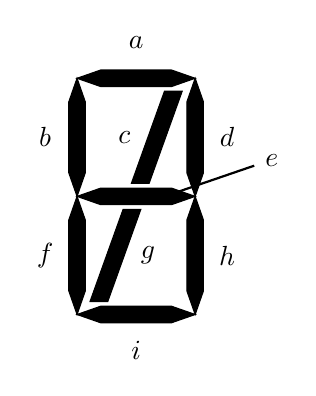
\begin{tikzpicture}
\begin{scope}[scale=0.15]
\path[draw,fill]%
(-5,1)--(-3,1.7)--(3,1.7)--(5,1)--(3,0.3)--(-3,0.3)--cycle;
\path[draw,fill]%
(-5,11)--(-3,11.7)--(3,11.7)--(5,11)--(3,10.3)--(-3,10.3)--cycle;
\path[draw,fill]%
(-5,21)--(-3,21.7)--(3,21.7)--(5,21)--(3,20.3)--(-3,20.3)--cycle;
\path[draw,fill]%
(5,1)--(4.3,3)--(4.3,9)--(5,11)--(5.7,9)--(5.7,3)--cycle;
\path[draw,fill]%
(5,11)--(4.3,13)--(4.3,19)--(5,21)--(5.7,19)--(5.7,13)--cycle;
\path[draw,fill]%
(-5,11)--(-4.3,13)--(-4.3,19)--(-5,21)--(-5.7,19)--(-5.7,13)--cycle;
\path[draw,fill]%
(-5,1)--(-4.3,3)--(-4.3,9)--(-5,11)--(-5.7,9)--(-5.7,3)--cycle;
\path[draw,fill]%
(3.9,19.9)--(2.4,19.9)--(-0.4,12.1)--(1.1,12.1)--cycle;
\path[draw,fill]%
(-3.9,2.1)--(-2.4,2.1)--(0.4,9.9)--(-1.1,9.9)--cycle;
\path[draw,thick](3,11.2)--(10,13.6);
\node at (0,24)    {$a$};
\node at (-7.7,16) {$b$};
\node at (-1,16)   {$c$};
\node at (7.7,16)  {$d$};
\node at (11.5,14) {$e$};
\node at (-7.7,6)  {$f$};
\node at (1,6)     {$g$};
\node at (7.7,6)   {$h$};
\node at (0,-2)    {$i$};
\end{scope}
\end{tikzpicture}
\end{minipage}
\qquad \qquad
\begin{minipage}{0.56\textwidth}
$\begin{array}{|ccc|ccccccccc|}
   X & Y & Z & a & b & c & d & e & f & g & h & i
\\ \hline
   0 & 0 & 0 & 1 & 1 & 0 & 1 & 0 & 1 & 0 & 1 & 1
\\ 0 & 0 & 1 & 0 & 0 & 1 & 1 & 0 & 0 & 0 & 1 & 0
\\ 0 & 1 & 0 & 1 & 0 & 0 & 1 & 1 & 1 & 0 & 0 & 1
\\ 0 & 1 & 1 & 1 & 0 & 1 & 0 & 1 & 0 & 0 & 1 & 1
\\ 1 & 0 & 0 & 0 & 1 & 0 & 1 & 1 & 0 & 0 & 1 & 0
\\ 1 & 0 & 1 & 1 & 1 & 0 & 0 & 1 & 0 & 0 & 1 & 1
\\ 1 & 1 & 0 & 1 & 1 & 0 & 0 & 1 & 1 & 0 & 1 & 1
\\ 1 & 1 & 1 & 1 & 0 & 1 & 0 & 0 & 0 & 1 & 0 & 0
\\ \hline
\multicolumn{12}{c}{~}
\end{array}$
\end{minipage}

\noindent
The single-digit display must be implemented with logic circuitry.
Here we assume that only three types of logic gates are available.
An \emph{and-gate} takes two inputs and produces, as output, the
conjunction ($\land$) of the inputs.
Similarly, an \emph{or-gate} implements disjunction ($\lor$).
Finally, an \emph{inverter} takes a single input and negates it.

The task here is to design a circuit for all of $a$--$i$ using as
few gates as possible.
We can specify the circuit by writing down the Boolean equations
for each of the outputs $a$--$i$.
For example, we can define $c = (\neg X \lor Y) \land Z$, which shows
that $c$ can be implemented with just three gates.
Since we want to use as few gates as possible, it is important to
look for cases where outputs can be \emph{shared}, or reused.
For example, $g$ can clearly be implemented with two and-gates,
but if we already have implemented $c$ then we could instead
define $g = c \land X$, using just one gate.
Note that any sub-circuit that you want to share (that is, you
want to direct its output to different places), the output must
have a name.
You can define as many ``helper'' functions as you please, to
create the smallest possible solution.

The answer to this question must be submitted separately on Grok
(details below).
Submit a text file consisting of one line per definition.
This file will be tested automatically, so it is important that
you follow the notational conventions exactly.
We write $\neg$ as \texttt{-} and $\lor$ as \texttt{+}.
We write $\land$ as \texttt{.}, or, simpler, we just leave it out,
so that concatenation of expressions denotes their conjunction.
Here is an example set of equations (for a different problem):
\begin{verbatim}
    # An example of a set of equations in the correct format:
    a = -Y Z + Y -Z + X -Y -Z
    b = u + X (Y + Z)
    c = X + -(Y Z)
    d = u + X a
    u = -X -Y
    # u is an auxiliary function introduced to simplify b and d
\end{verbatim}
Empty lines, and lines that start with `\#', are ignored.
Input variables are in upper case.
Negation binds tighter than conjunction, which in
turn binds tighter than disjunction.
So the equation for $a$ says that
$a = (\neg Y \land Z) \lor (Y \land \neg Z) \lor (X \land \neg Y \land \neg Z)$.
Note the use of a helper function $u$, allowing $b$ and $d$ to
share some circuitry.
Also note that we do not allow any feedback loops in the circuit.
In the example above, $d$ depends on $a$, so $a$ is not allowed
to depend, directly or indirectly, on $d$ (and indeed it does not).

\section*{Submission and assessment}
Some of the problems are harder than others.
All should be solved and submitted by students individually.
Your solution will count for 12 marks out of 100 for the subject.
Each question is worth 2~marks.
Marks are primarily allocated for correctness, but elegance and how
clearly you communicate your thinking will also be taken into account.
For Challenge 6, there will be 1 mark for a correct solution. 
After that, your mark depends on which quartile your solution sits in, 
when we order all solutions by increasing number of gates.
If it falls in the best quartile (that is, within the 25\% of
solutions that use the fewest gates), we add 1 mark.
If you are in the next quartile, we add 0.5 marks.
Otherwise no marks are added to the mark for correctness.

The deadline is 9 September at 23:00.
Late submission will be possible, but a late submission penalty will
apply: a flagfall of 1 mark, and then 1 mark per 12 hours late.

\emph{For all challenges except number 6}, submit a PDF document via the LMS.
This document should be no more than 1 MB in size.
If you produce an MS Word document, it must be exported
and submitted as PDF, and satisfy the space limit of 1 MB.
We also accept \emph{neat} hand-written submissions, but these must be
scanned and provided as PDF, and again, they must respect the size limit.
If you scan your document, make sure you set the resolution so that
the generated document is no more than 1 MB.

Being neat is easier if you type-set your answers, but not all
typesetting software does a good job of presenting mathematical formulas.
The best tool for this is \LaTeX, which is worth learning if you expect
that you will later have to produce large technical documents.
Admittedly, diagrams are tedious to do with \LaTeX,
even when using sophisticated packages such as Tikz.
You could, of course, mix typeset text with hand-drawn diagrams.
In case you want to use the assignment to get some \LaTeX\ practice,
I will leave the source for this document in the
content area where you find the PDF version.

\emph{For challenge 6}, submit a text file on Grok.
You will receive immediate feedback from an elementary test,
which checks that your input has the correct format, 
and that it implements the desired circuit correctly.
Note that on Grok, ``saving'' your file does not mean 
submitting it for marking. 
To submit, you need to click ``mark''.
You can submit as many times as you like.
What gets marked is the last submission you have made before the deadline.

Make sure that you have enough time towards the end of the assignment
to present your solutions carefully.
A nice presentation is sometimes more time consuming than solving the
problems.
Start early; note that time you put in early usually turns out more
productive than a last-minute effort.
For Challenge 6 in particular, you don't want to submit ``improved''
solutions a few minutes before the deadline, as they may turn out
to be wrong and you won't have time to fix this.

Individual work is expected, but if you get stuck, email Matt or Harald
a precise description of the problem, bring up the problem at the
lecture, or (our preferred option) use the LMS discussion board.
The COMP30026 LMS discussion forum is both useful and appropriate
for this;
soliciting help from sources other than the above
will be considered cheating and will lead to disciplinary action.

\begin{flushright}
Harald S{\o}ndergaard
\\ 23 August 2018, revised 27 and 28 August
\end{flushright}

\end{document}
